\documentclass[landscape]{article}
\usepackage{amssymb}
\usepackage[landscape]{geometry}
\usepackage{multicol}
%\usepackage{helvet}
\usepackage{color}
%\usepackage[xdvi,dvips]{graphicx}
\usepackage{graphicx}
\usepackage{amsfonts, amstext, amsmath}
\usepackage{wrapfig}
\usepackage{float}
\usepackage[export]{adjustbox}
\usepackage{tcolorbox}
\usepackage{times}
\usepackage{anyfontsize}
\usepackage{tikz}
\usepackage{graphicx}
\usetikzlibrary{calc}
\usepackage{listings}

\newtcolorbox{mybox}{boxrule=6pt}

\def\argmax{\qopname\relax n{argmax}}
\def\s{\mathbf s}
\def\x{\mathbf x}
\def\u{\mathbf u}
\def\y{\mathbf y}
\def\d{\mathbf d}
\def\boldzero{\mathbf 0}
\def\pibold{\mbox{\boldmath $\pi$}}
\newcommand{\normal}[2]{\ensuremath{\mathcal{N}\left(#1,#2\right)}}
\newcommand{\given}{\mid}

\newenvironment{itemizeNoSymbol}{%
\renewcommand{\labelitemi}{}\begin{itemize}
\setlength{\itemsep}{1pt}
\setlength{\parskip}{0pt}
\setlength{\parsep}{0pt}}{\end{itemize}}


% set horizontal margins to center text (using current paperwidth &
% textwidth)
\newcommand{\equalmargins} {
\setlength{\oddsidemargin}{\paperwidth}
\addtolength{\oddsidemargin}{-\textwidth}
\setlength{\oddsidemargin}{0.5 \oddsidemargin}
\addtolength{\oddsidemargin}{-1in}
}

\setlength{\evensidemargin}{\oddsidemargin}

\renewcommand{\familydefault}{\sfdefault}

\input posterfonts.tex

% setup large (poster-sized) sheet
\setlength{\paperwidth}{180cm}
\setlength{\paperheight}{105cm}
%\pdfpagewidth\paperwidth
%\pdfpageheight\paperheight
 
\setlength{\textwidth}{175cm}
\setlength{\textheight}{100cm}
\setlength{\topmargin}{-.25truein}
 
\equalmargins
\setlength{\headsep}{0pt}
\setlength{\headheight}{0pt}

\pagestyle{empty}
\setlength{\parindent}{0mm}
\setlength{\parskip}{16pt}

% header style: title followed by a column-wide rule
\newcommand{\mysection}[1]{{\color[rgb]{.6,0,0}{\section*{{\HUGE #1}
        {\leaders\hrule height .2ex\hfill\kern0pt}}}}}

\begin{document}
\color{black}

% invisible rule is useful for spacing
\hrule width 0pt depth 0pt height 1pt

\begin{center}
  \titleSize
Analyzing the role of task-selective connectivity in superior colliculus using EPI \\
  \HUGE %
  Sean R. Bittner$^{1}$, Alex T. Piet $^{2}$, Chunyu A. Duan$^{3}$, Carlos D. Brody $^{4}$, and John P. Cunningham$^5$ \\
\huge
 $^{1}$Department of Neuroscience, Columbia University, $^{2}$ Allen Institute for Brain Science, $^{3}$ Institute of Neuroscience, Chinese Academy of Sciences, \\ $^{4}$ Princeton Neuroscience Institute, and $^{5}$Department of Statistics, Columbia University
\end{center}

\begin{tikzpicture}[remember picture,overlay]
  \node[anchor=north east,inner sep=-0pt, scale=1.5] at ($(current page.north east)+(-1cm,-1cm)$) {
     \includegraphics{figs/CU_logo}
  };
\end{tikzpicture}

%%%%%%%%%%%%%%%%%%%%%%%%%%%%%%
\begin{minipage}[c]{0.29\linewidth}
\vspace{-1in}
\mysection{Motivation}
\LARGE
\begin{itemize}
\item Experimental evidence suggests superior colliculus (SC) is a principal contributor to flexible routing in rats.
\item Neural response properties in SC motivate a circuit model with functionally-defined neuron-type populations.
\item We use emergent property inference (EPI) to reveal the role of connectivity properties of SC in rapid task switching.
\end{itemize}
\vspace{-.25in}
\mysection{Methods}
{\huge \textbf{Emergent property inference (EPI)}} \\
\vspace{-.5in}
\begin{itemize}
\item EPI enables statistical inference in a broad class of neural circuit models by leveraging the modern inference engine.
\end{itemize}
\begin{multicols*}{2}
\begin{center}
\adjincludegraphics[clip, trim={0 0 0 0},scale=1.3]{figs/DSN.pdf}
\end{center}
\columnbreak
\begin{itemize}
\item Deep probability distributions are obtained by optimizing deep networks to map (approximately) a simple random distribution to a target dist.
\[z = f_l \circ f_{l-1} \circ ... \circ f_1 \circ \omega \]
\end{itemize}
\end{multicols*}
\begin{itemize}
\item With EPI [1], we use deep learning to obtain distributions of model parameters producing emergent properties of computation. \vspace{1cm} \\
\textbf{Example: stomatogastric ganglion (STG)}
\begin{center}
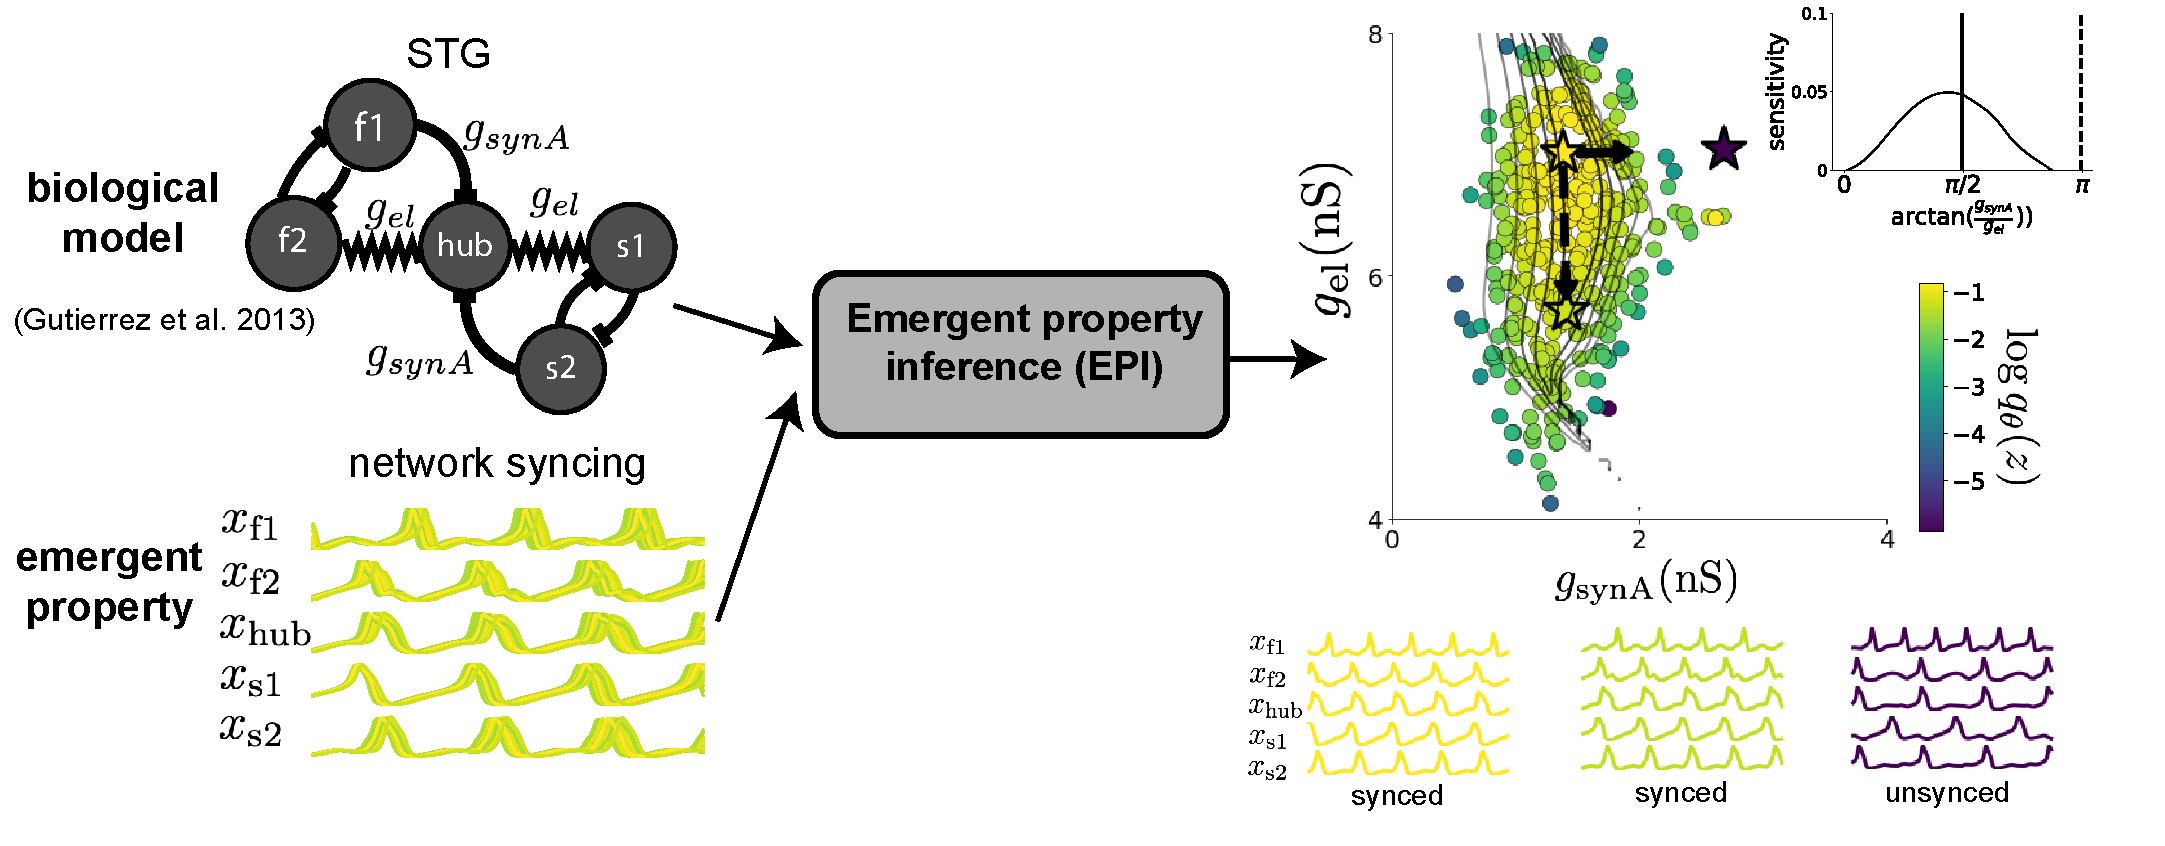
\includegraphics[scale=1.4]{figs/Cosyne2020fig1.pdf}
\end{center}
\textbf{Optimization}:
\item In EPI, probability distributions of parameters $z \sim q_\theta(z)$ are optimized to produce emergent property $\mathcal{B}: E_{z \sim q_\theta(z)} \left[ E_{p(x \mid z)} \left[T(x) \right] \right] = \mu$, given a choice of model $p(x \mid z)$ and emergent property $\mathcal{B}$. \\
\begin{center}
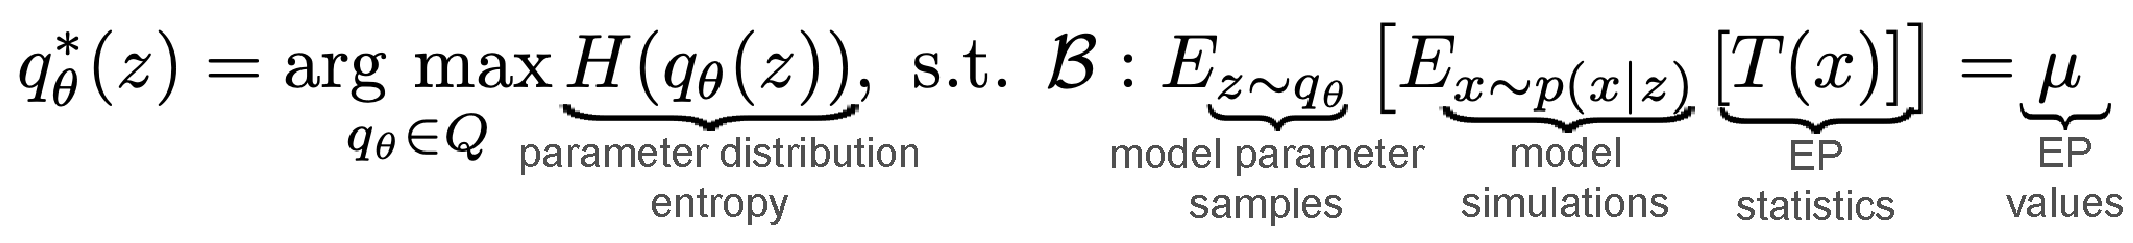
\includegraphics[scale=1.25]{figs/EPI_opt.pdf}
\end{center}
\end{itemize}
\end{minipage}
\hspace{1cm} \begin{minipage}[c]{0.36\linewidth}
%%%%%%%%%%%%%%%%%%%%%%%%%%%%%%
\mysection{Flexible task switching}
\LARGE
\begin{multicols*}{2}
\begin{itemize}
\item Rats were trained to rapidly switch between tasks (Pro/Anti). Optogenetic inactivation of SC during the delay diminishes performance.
\vspace{.25cm}
\begin{center}
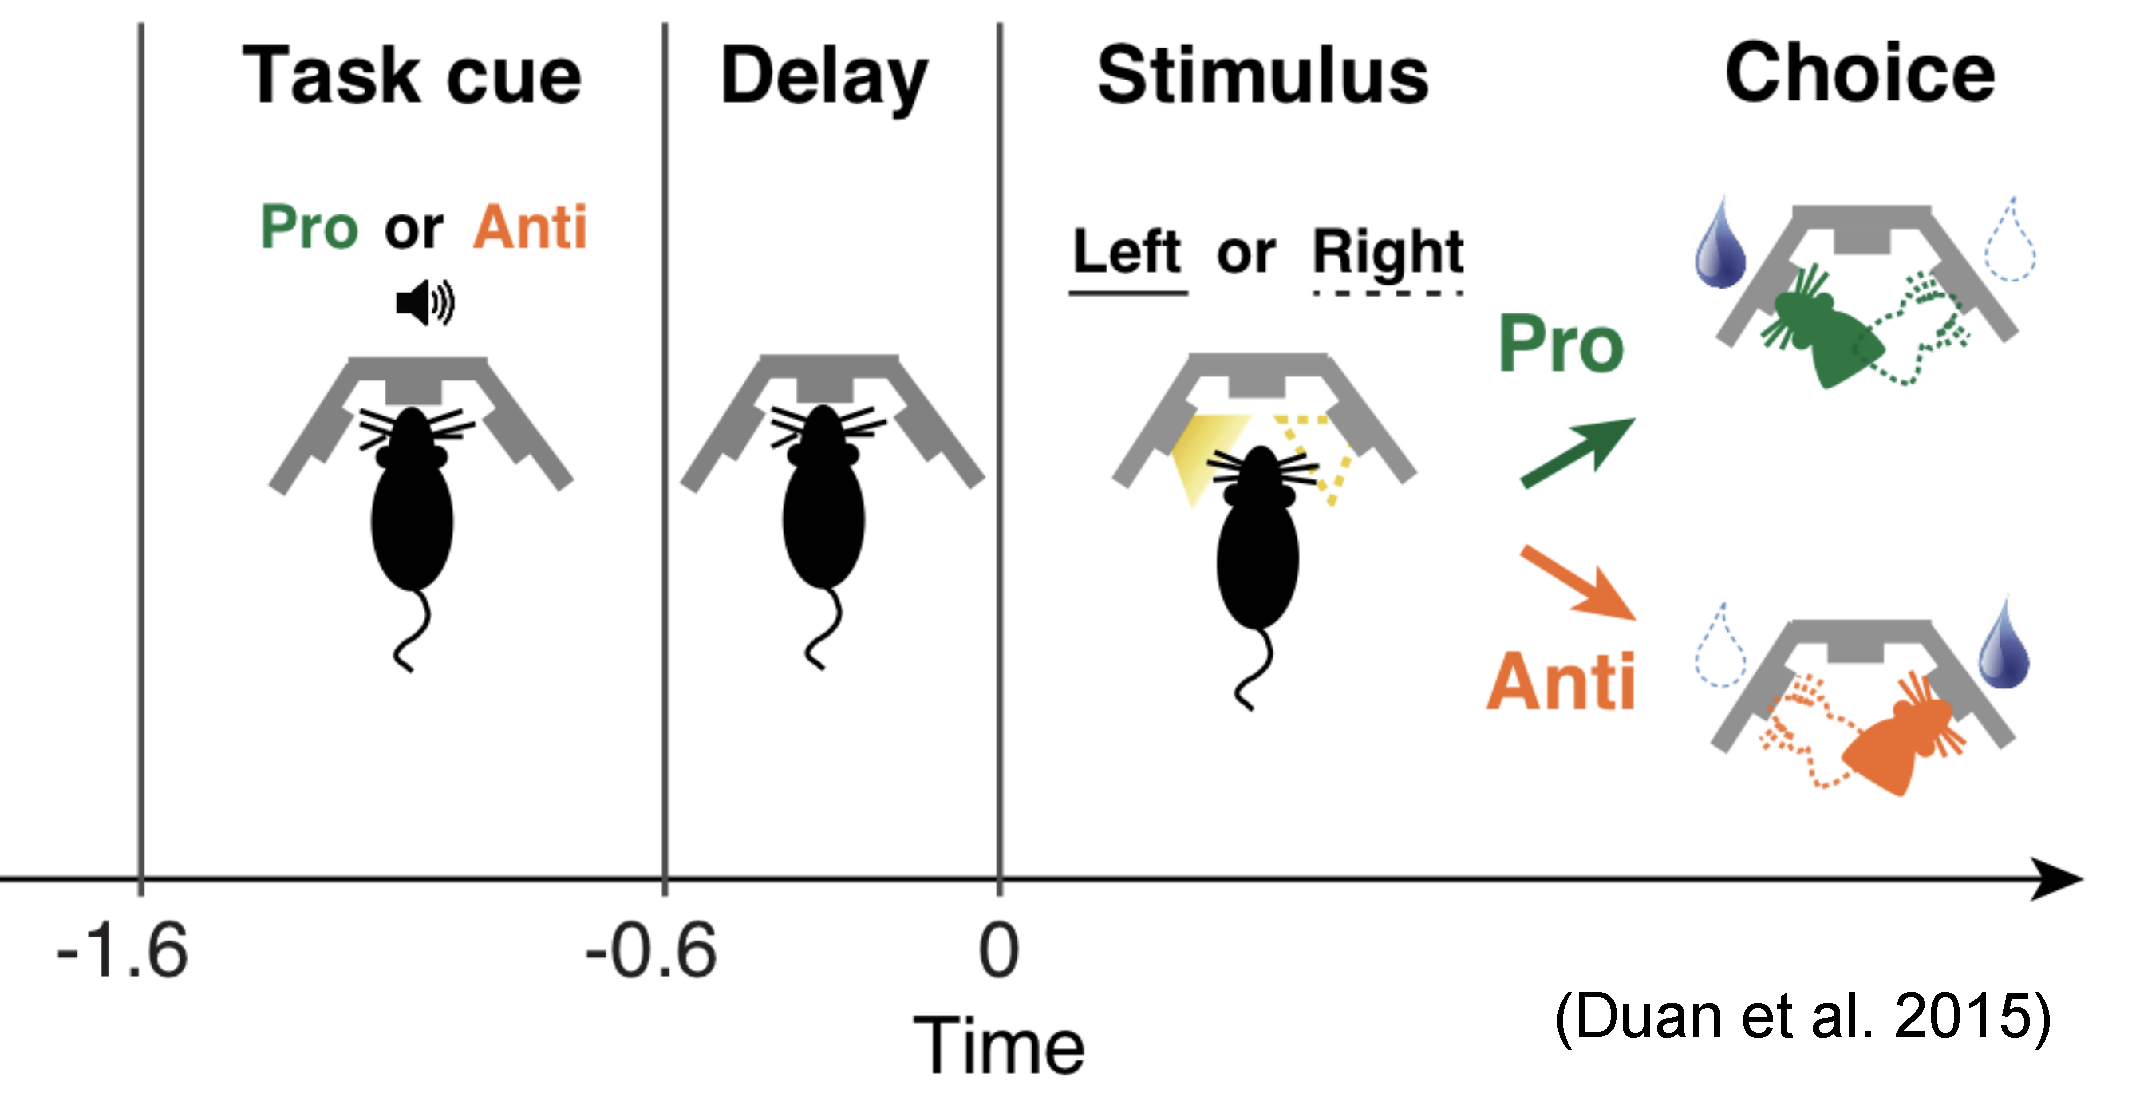
\includegraphics[scale=0.75]{figs/Duan2018Task.pdf} \\
\end{center}
\item SC neurons are strongly tuned to Pro/Anti.
\end{itemize}
\columnbreak
\begin{center}
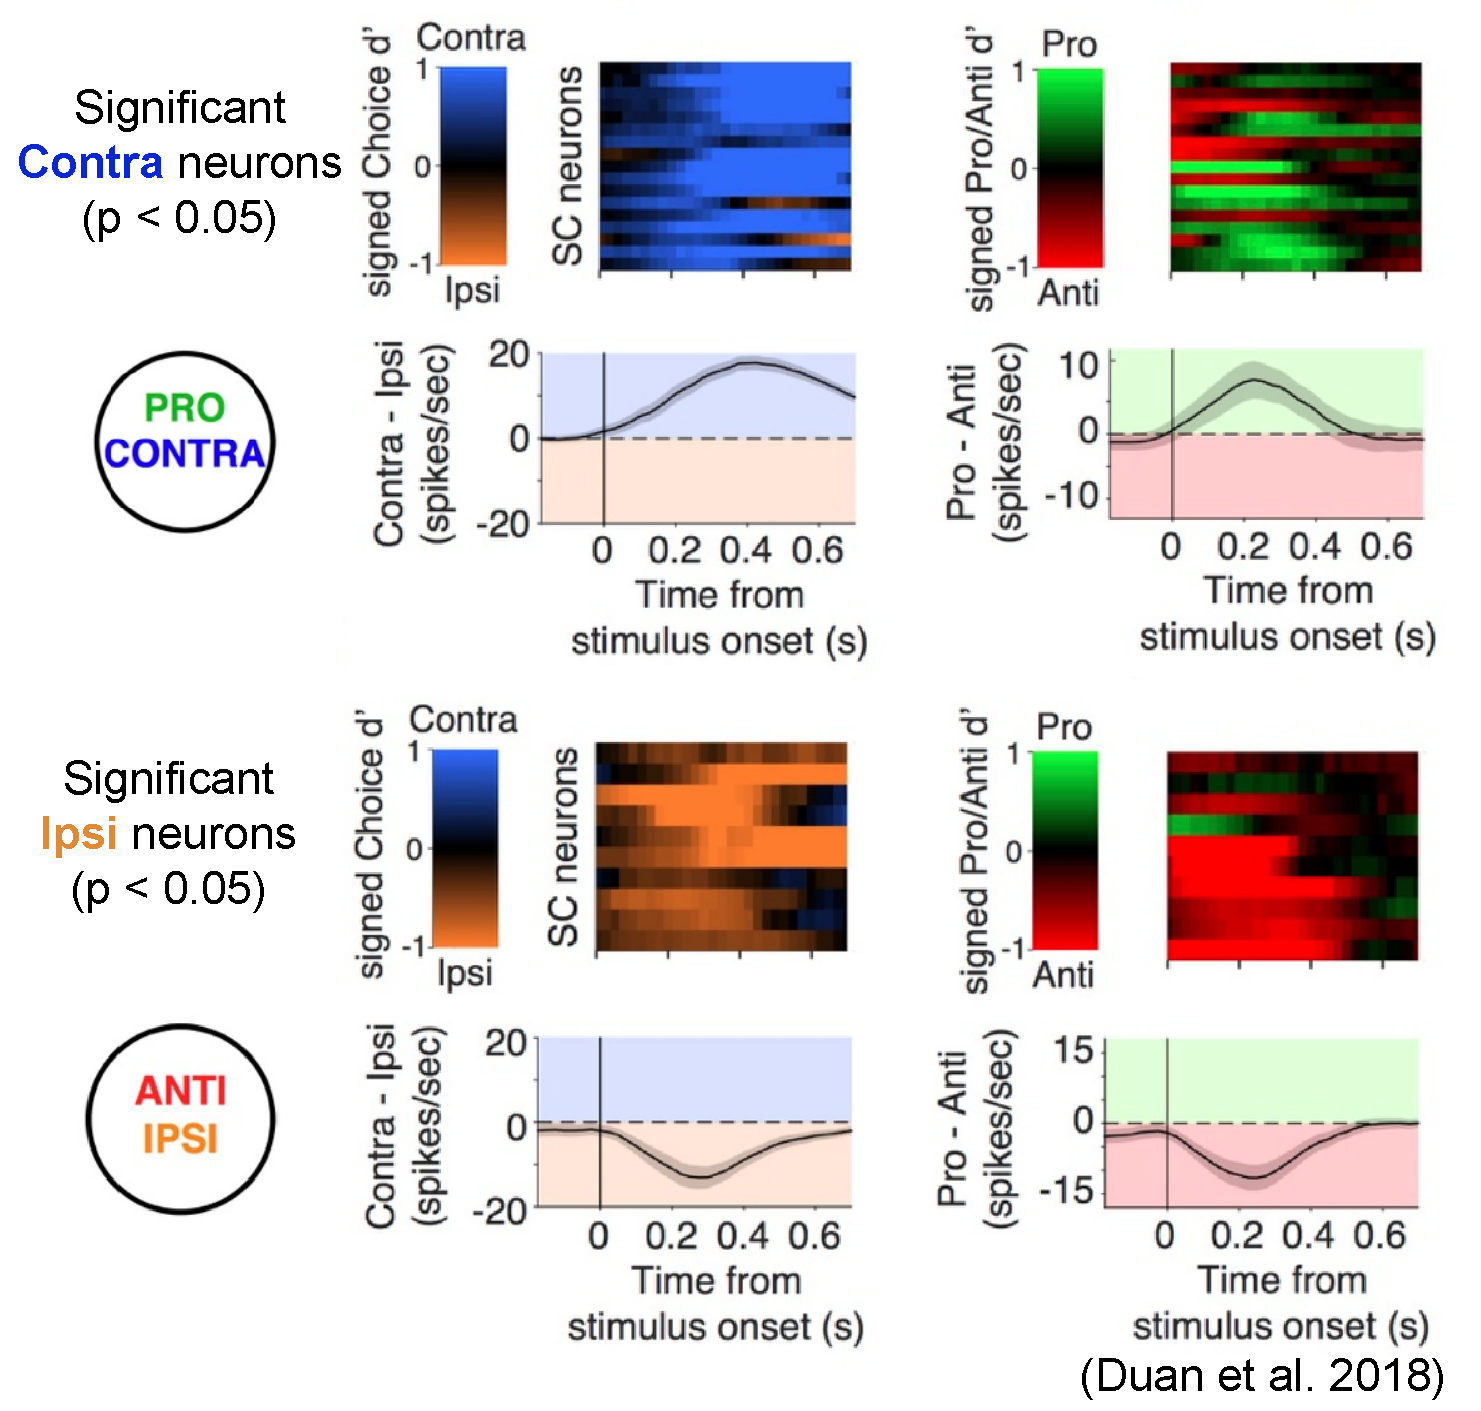
\includegraphics[scale=.95]{figs/pro_contra.pdf}
\end{center}
\end{multicols*}
\begin{itemize}
\item Such Pro/Anti neurons are also strongly tuned to Contra/Ipsi responses, respectively.
\end{itemize}
\vspace{.5cm}
\textbf{SC model executing rapid task switching} (Duan et al. 2018):\\
\vspace{-2cm}
\begin{center}
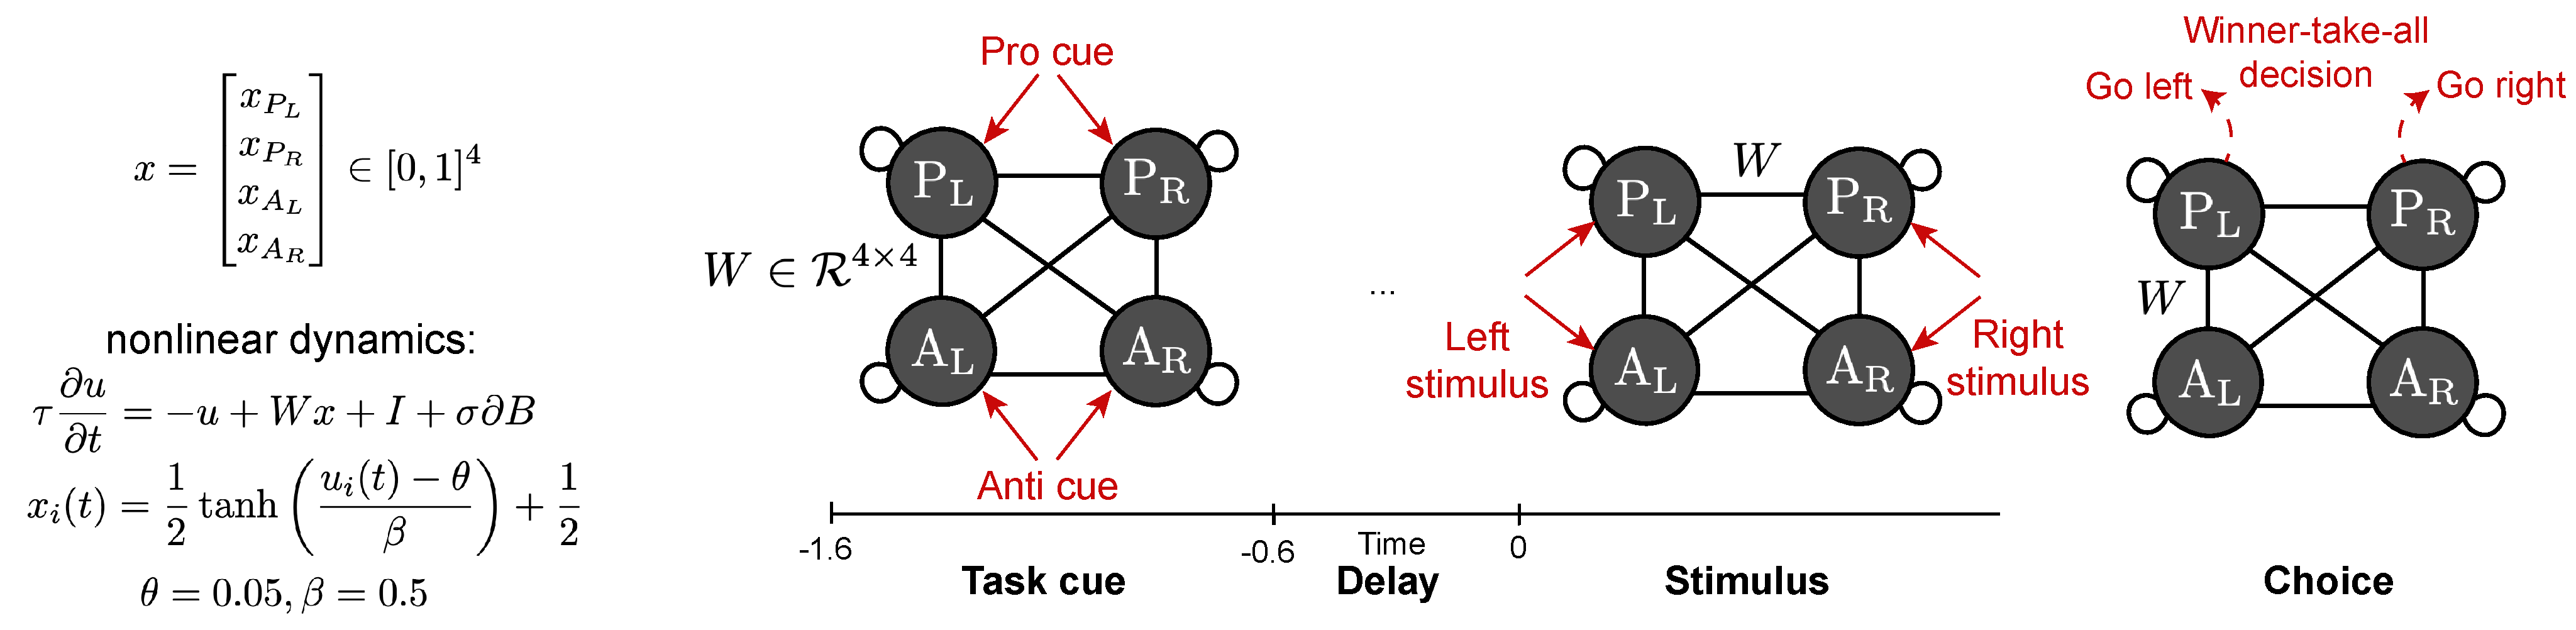
\includegraphics[scale=0.8]{figs/SC_model.pdf}
\end{center}
\textbf{Schur connectivity decomposition:}\\
\includegraphics[scale=2.0]{figs/SC_Schur.pdf}
\mysection{Inference of connectivity given task accuracy}
\LARGE
\begin{itemize}
\item Using EPI, we infer connectivity distributions consistent with various levels of accuracy.
\end{itemize}
\begin{center}
\vspace{1cm}
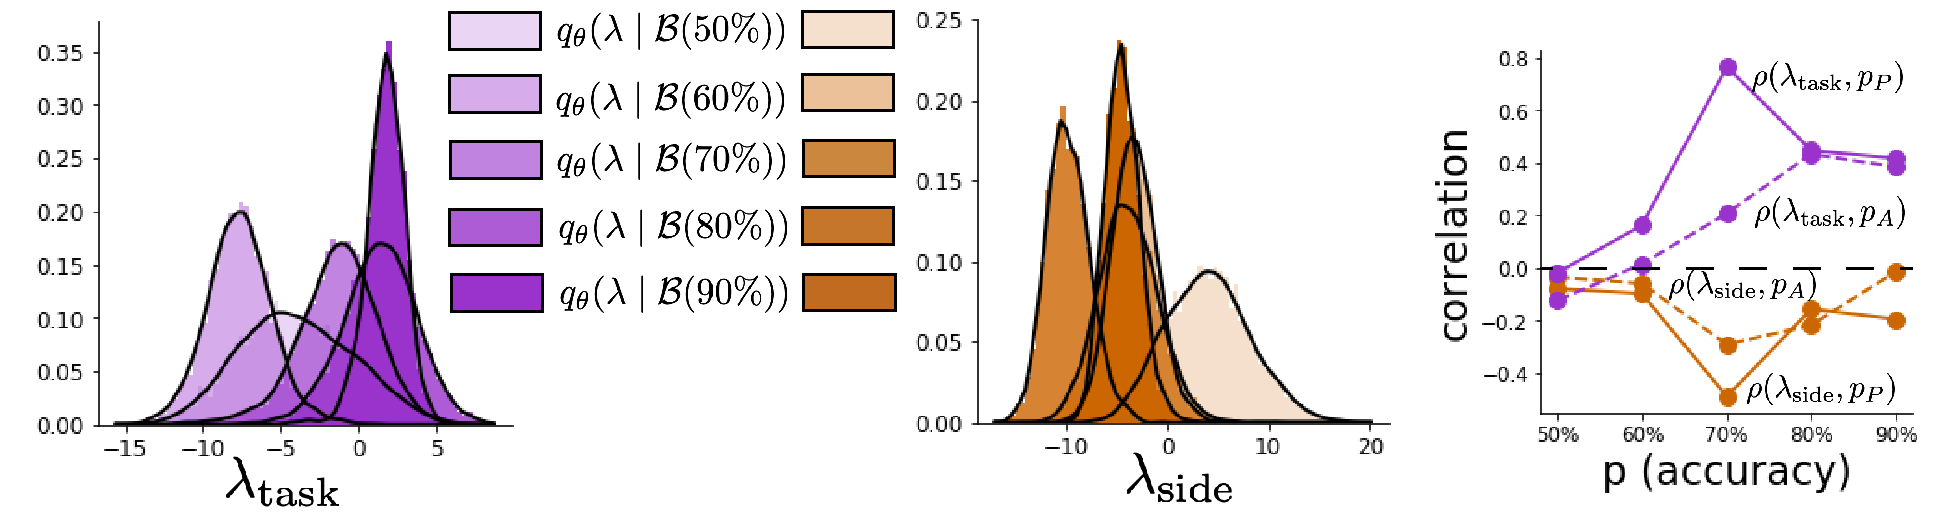
\includegraphics[scale=1.4]{figs/SC_Fig4.pdf}
\end{center}
\begin{itemize}
\item With greater accuracy, the task mode is amplified, and the side mode is suppressed.
\item This reveals the importance of task representation and hemispheric balance in connectivity of rapid task switching networks.
\end{itemize}

\end{minipage}
\hspace{1cm} \begin{minipage}[c]{0.29\linewidth}
%%%%%%%%%%%%%%%%%%%%%%%%%%%%%%
\LARGE
\begin{itemize}
\item Visualizing the EPI  distributions at each accuracy level, including additional distributions of $\lambda_{\text{task}}$ at additional random seeds, further supports the concluded trend of $\lambda_{\text{task}}$ with accuracy.
\vspace{-1in}
\end{itemize}
\begin{center}
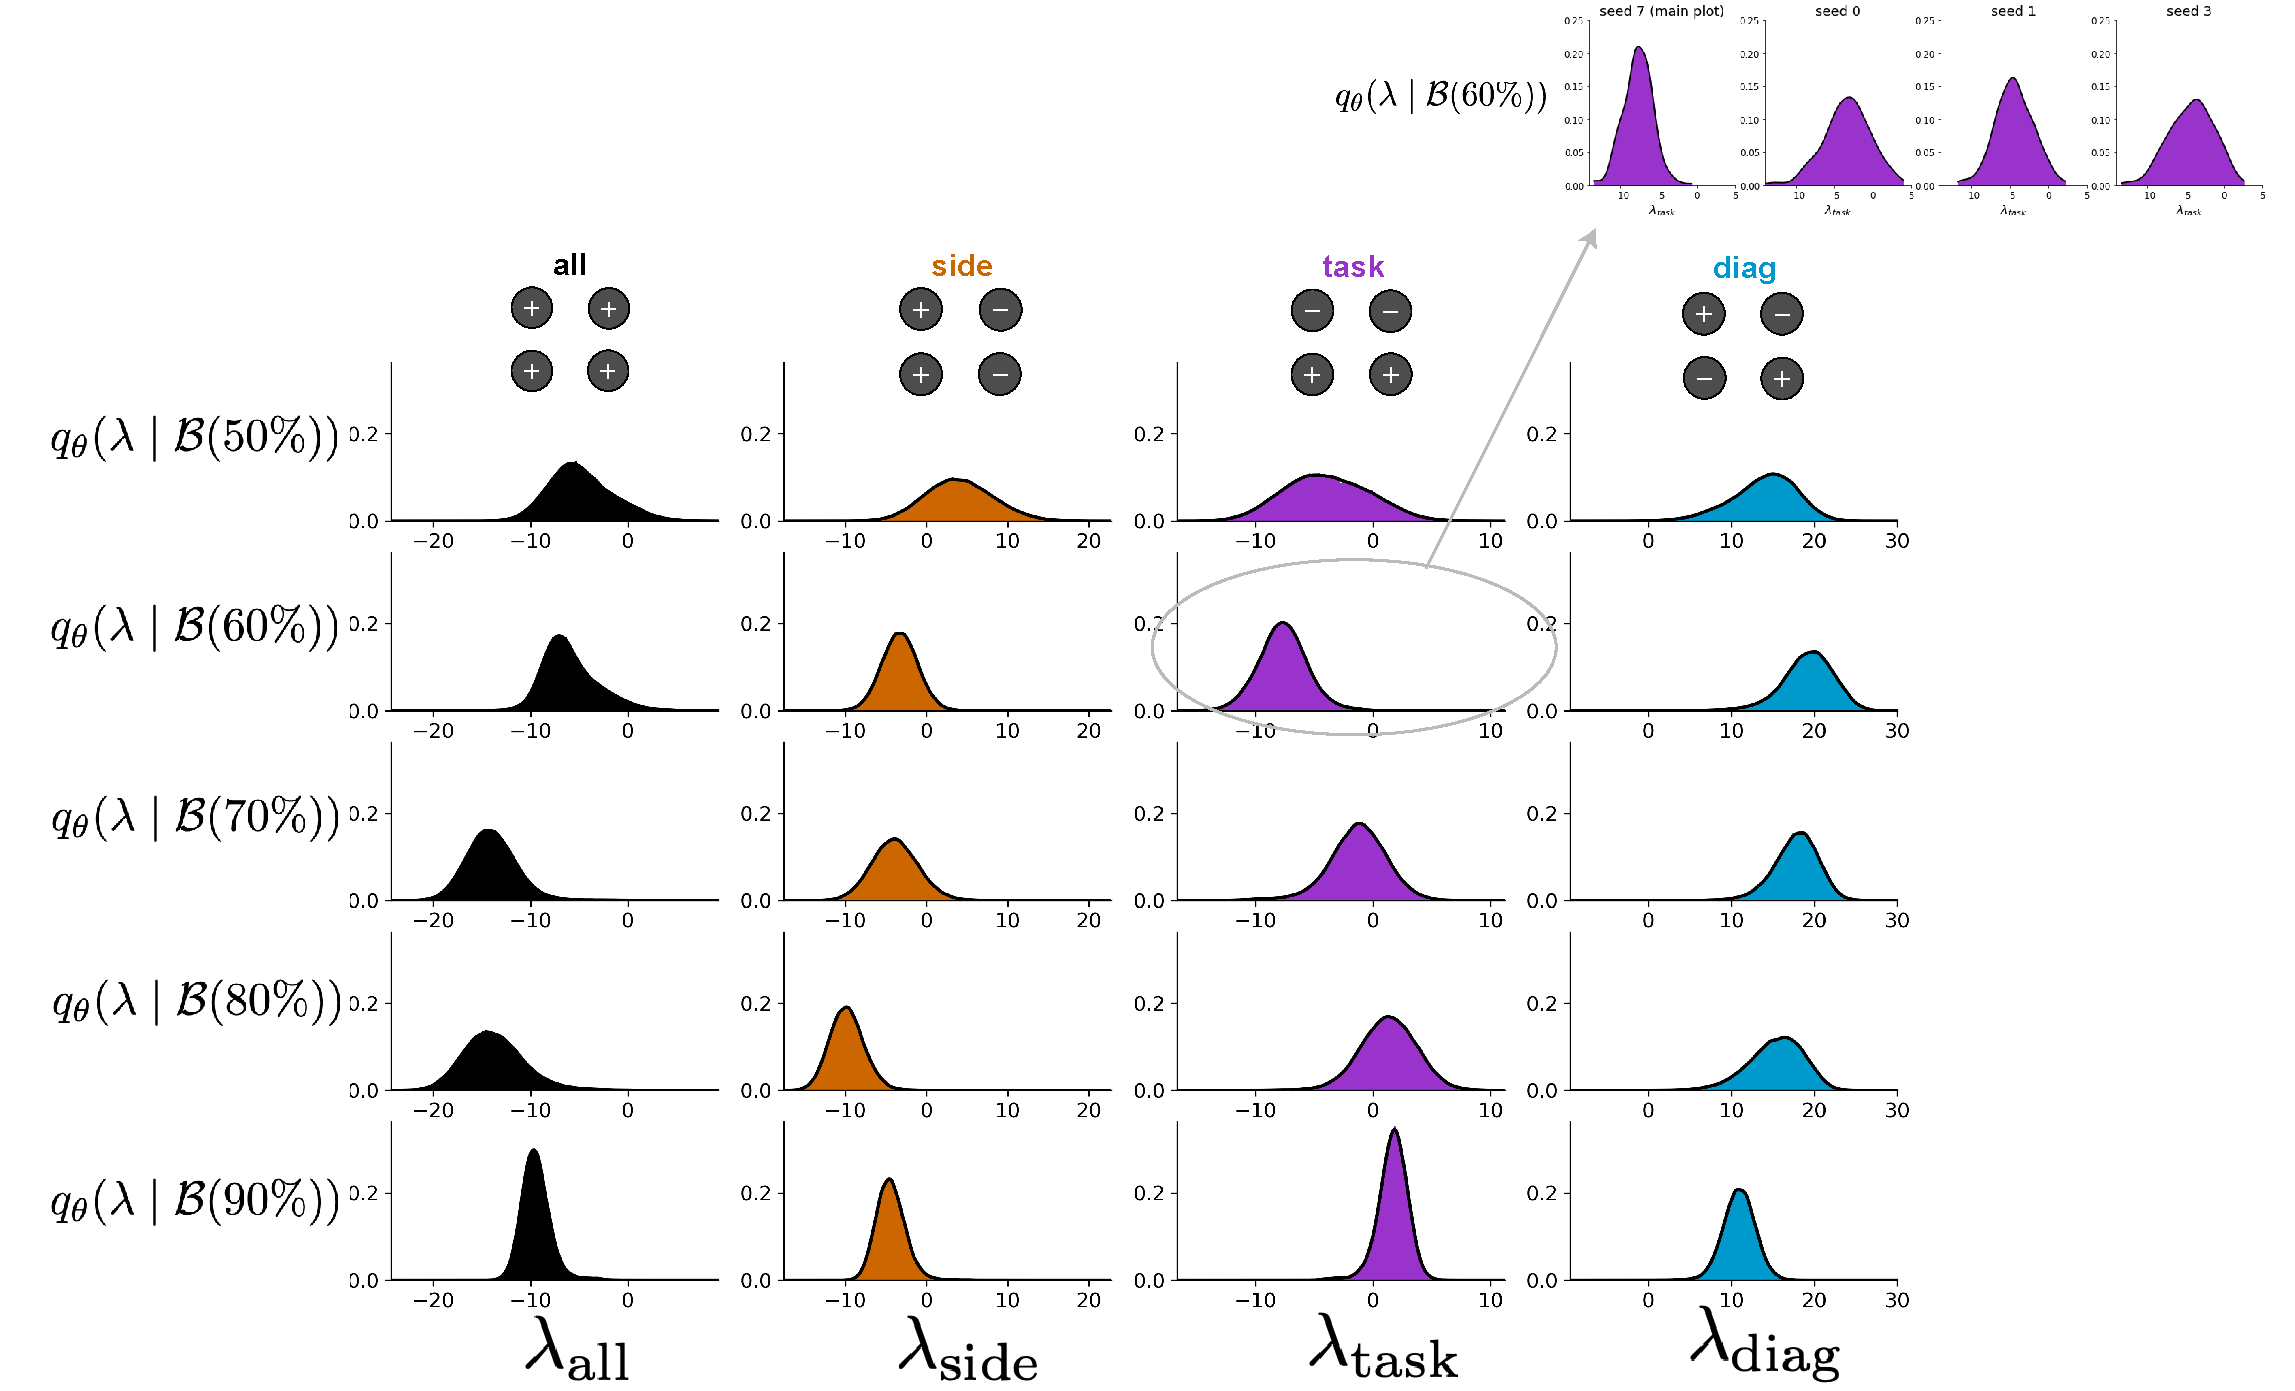
\includegraphics[scale=1.2]{figs/SC_results.pdf}
\end{center}

\mysection{Summary}
\begin{itemize}
\item We used EPI to characterize how effective connectivity governs task accuracy in a complex nonlinear dynamical model.
\item We produce experimental predictions that specific, interpretable patterns of effective connectivity will correlate with higher rapid task switching accuracy. 
\item The approach taken with EPI can be applied generally to biophysical models, nonlinear sensory models, as well as infinite-size RNNs [1].
\end{itemize}

\mysection{Code availability}
To run EPI on your neural circuit model:
\begin{enumerate}
\item Write a python function of the emergent property given model parameters.
\item The \texttt{epi} python package will do the rest. \\
\texttt{git clone https://github.com/cunningham-lab/epi.git}
\end{enumerate}
\vspace{1cm}

{\bf\LARGE References} \\
\large
1. Bittner, Sean R., et al. "Interrogating theoretical models of neural computation with deep inference." bioRxiv (2019): 837567. \\
2. Gutierrez, Gabrielle J., Timothy O’Leary, and Eve Marder. "Multiple mechanisms switch an electrically coupled, synaptically inhibited neuron between competing rhythmic oscillators." Neuron 77.5 (2013): 845-858.  \\
3. Duan, Chunyu A. et al. "Requirement of prefrontal and midbrain regions for rapid executive control of behavior in the rat." Neuron 86.6 (2015): 1491-1503.\\
4. Duan, Chunyu A., et al. "Collicular circuits for flexible sensorimotor routing." bioRxiv (2018): 245613. \\
{\bf\large Acknowledgements} \\
\large
NSF Grad. Research Fellowship,  DGE-1644869, McKnight Endowment Fund, NIH NINDS 5R01NS100066, Simons Foundation. 542963, NSF 1707398, The Gatsby Charitable Foundation. Stephen Baccus, James Fitzgerald, Dhruva Raman, Francesca Mastrogiuseppe, and Srdjan Ostojic for helpful conversations. \\
\end{minipage}

\end{document}
